\documentclass[]{article}
\usepackage{lmodern}
\usepackage{amssymb,amsmath}
\usepackage{ifxetex,ifluatex}
\usepackage{fixltx2e} % provides \textsubscript
\ifnum 0\ifxetex 1\fi\ifluatex 1\fi=0 % if pdftex
  \usepackage[T1]{fontenc}
  \usepackage[utf8]{inputenc}
\else % if luatex or xelatex
  \ifxetex
    \usepackage{mathspec}
  \else
    \usepackage{fontspec}
  \fi
  \defaultfontfeatures{Ligatures=TeX,Scale=MatchLowercase}
\fi
% use upquote if available, for straight quotes in verbatim environments
\IfFileExists{upquote.sty}{\usepackage{upquote}}{}
% use microtype if available
\IfFileExists{microtype.sty}{%
\usepackage{microtype}
\UseMicrotypeSet[protrusion]{basicmath} % disable protrusion for tt fonts
}{}
\usepackage[a4paper, margin=25mm, portrait]{geometry}
\usepackage{hyperref}
\hypersetup{unicode=true,
            pdfborder={0 0 0},
            breaklinks=true}
\urlstyle{same}  % don't use monospace font for urls
\usepackage{color}
\usepackage{fancyvrb}
\newcommand{\VerbBar}{|}
\newcommand{\VERB}{\Verb[commandchars=\\\{\}]}
\DefineVerbatimEnvironment{Highlighting}{Verbatim}{commandchars=\\\{\}}
% Add ',fontsize=\small' for more characters per line
\usepackage{framed}
\definecolor{shadecolor}{RGB}{248,248,248}
\newenvironment{Shaded}{\begin{snugshade}}{\end{snugshade}}
\newcommand{\KeywordTok}[1]{\textcolor[rgb]{0.13,0.29,0.53}{\textbf{{#1}}}}
\newcommand{\DataTypeTok}[1]{\textcolor[rgb]{0.13,0.29,0.53}{{#1}}}
\newcommand{\DecValTok}[1]{\textcolor[rgb]{0.00,0.00,0.81}{{#1}}}
\newcommand{\BaseNTok}[1]{\textcolor[rgb]{0.00,0.00,0.81}{{#1}}}
\newcommand{\FloatTok}[1]{\textcolor[rgb]{0.00,0.00,0.81}{{#1}}}
\newcommand{\ConstantTok}[1]{\textcolor[rgb]{0.00,0.00,0.00}{{#1}}}
\newcommand{\CharTok}[1]{\textcolor[rgb]{0.31,0.60,0.02}{{#1}}}
\newcommand{\SpecialCharTok}[1]{\textcolor[rgb]{0.00,0.00,0.00}{{#1}}}
\newcommand{\StringTok}[1]{\textcolor[rgb]{0.31,0.60,0.02}{{#1}}}
\newcommand{\VerbatimStringTok}[1]{\textcolor[rgb]{0.31,0.60,0.02}{{#1}}}
\newcommand{\SpecialStringTok}[1]{\textcolor[rgb]{0.31,0.60,0.02}{{#1}}}
\newcommand{\ImportTok}[1]{{#1}}
\newcommand{\CommentTok}[1]{\textcolor[rgb]{0.56,0.35,0.01}{\textit{{#1}}}}
\newcommand{\DocumentationTok}[1]{\textcolor[rgb]{0.56,0.35,0.01}{\textbf{\textit{{#1}}}}}
\newcommand{\AnnotationTok}[1]{\textcolor[rgb]{0.56,0.35,0.01}{\textbf{\textit{{#1}}}}}
\newcommand{\CommentVarTok}[1]{\textcolor[rgb]{0.56,0.35,0.01}{\textbf{\textit{{#1}}}}}
\newcommand{\OtherTok}[1]{\textcolor[rgb]{0.56,0.35,0.01}{{#1}}}
\newcommand{\FunctionTok}[1]{\textcolor[rgb]{0.00,0.00,0.00}{{#1}}}
\newcommand{\VariableTok}[1]{\textcolor[rgb]{0.00,0.00,0.00}{{#1}}}
\newcommand{\ControlFlowTok}[1]{\textcolor[rgb]{0.13,0.29,0.53}{\textbf{{#1}}}}
\newcommand{\OperatorTok}[1]{\textcolor[rgb]{0.81,0.36,0.00}{\textbf{{#1}}}}
\newcommand{\BuiltInTok}[1]{{#1}}
\newcommand{\ExtensionTok}[1]{{#1}}
\newcommand{\PreprocessorTok}[1]{\textcolor[rgb]{0.56,0.35,0.01}{\textit{{#1}}}}
\newcommand{\AttributeTok}[1]{\textcolor[rgb]{0.77,0.63,0.00}{{#1}}}
\newcommand{\RegionMarkerTok}[1]{{#1}}
\newcommand{\InformationTok}[1]{\textcolor[rgb]{0.56,0.35,0.01}{\textbf{\textit{{#1}}}}}
\newcommand{\WarningTok}[1]{\textcolor[rgb]{0.56,0.35,0.01}{\textbf{\textit{{#1}}}}}
\newcommand{\AlertTok}[1]{\textcolor[rgb]{0.94,0.16,0.16}{{#1}}}
\newcommand{\ErrorTok}[1]{\textcolor[rgb]{0.64,0.00,0.00}{\textbf{{#1}}}}
\newcommand{\NormalTok}[1]{{#1}}
\usepackage{longtable,booktabs}
\usepackage{graphicx,grffile}
\makeatletter
\def\maxwidth{\ifdim\Gin@nat@width>\linewidth\linewidth\else\Gin@nat@width\fi}
\def\maxheight{\ifdim\Gin@nat@height>\textheight\textheight\else\Gin@nat@height\fi}
\makeatother
% Scale images if necessary, so that they will not overflow the page
% margins by default, and it is still possible to overwrite the defaults
% using explicit options in \includegraphics[width, height, ...]{}
\setkeys{Gin}{width=\maxwidth,height=\maxheight,keepaspectratio}
\IfFileExists{parskip.sty}{%
\usepackage{parskip}
}{% else
\setlength{\parindent}{0pt}
\setlength{\parskip}{6pt plus 2pt minus 1pt}
}
\setlength{\emergencystretch}{3em}  % prevent overfull lines
\providecommand{\tightlist}{%
  \setlength{\itemsep}{0pt}\setlength{\parskip}{0pt}}
\setcounter{secnumdepth}{0}
% Redefines (sub)paragraphs to behave more like sections
\ifx\paragraph\undefined\else
\let\oldparagraph\paragraph
\renewcommand{\paragraph}[1]{\oldparagraph{#1}\mbox{}}
\fi
\ifx\subparagraph\undefined\else
\let\oldsubparagraph\subparagraph
\renewcommand{\subparagraph}[1]{\oldsubparagraph{#1}\mbox{}}
\fi

%%% Use protect on footnotes to avoid problems with footnotes in titles
\let\rmarkdownfootnote\footnote%
\def\footnote{\protect\rmarkdownfootnote}

%%% Change title format to be more compact
\usepackage{titling}

% Create subtitle command for use in maketitle
\newcommand{\subtitle}[1]{
  \posttitle{
    \begin{center}\large#1\end{center}
    }
}

\setlength{\droptitle}{-2em}
  \title{}
  \pretitle{\vspace{\droptitle}}
  \posttitle{}
  \author{}
  \preauthor{}\postauthor{}
  \date{}
  \predate{}\postdate{}

\usepackage[fontsize=12pt]{scrextend}
\usepackage[utf8]{inputenc}
\renewcommand{\familydefault}{phv}
\usepackage{lineno}
\linenumbers
\usepackage{setspace}
\onehalfspacing
\raggedright

\begin{document}

\section{Building future landscapes to assess impact of land use land
cover change on provisioning of ecosystem
services}\label{building-future-landscapes-to-assess-impact-of-land-use-land-cover-change-on-provisioning-of-ecosystem-services}

\today  

Reto Schmucki\textsuperscript{1}

\textsuperscript{1} CEH, Benson Lane, MacLean Building, Wallingford,
OX10 8BB, UK

\subsubsection{Abstract}\label{abstract}

LULC change models (Schmucki \emph{et al.} 2016) may become fundamental
(Aquilué \emph{et al.} 2017) tools to accurately inform policy makers
and land managers committed to sustainable development, biodiversity
conservation \(\sqrt{27}\) and regional assessments of ecosystem
services provisioning.

\subsubsection{Introduction}\label{introduction}

Land use are dynamics and change in configuration (Phillips \emph{et
al.} 2017) and history of land use have important impact on provisioning
of \(X^2_{i,j}\) ecosystem services.

\begin{Shaded}
\begin{Highlighting}[]
\NormalTok{a <-}\StringTok{ }\DecValTok{2+4}
\NormalTok{b <-}\StringTok{ }\DecValTok{1}\NormalTok{/}\KeywordTok{sqrt}\NormalTok{(}\DecValTok{4}\NormalTok{)}
\NormalTok{c <-}\StringTok{ }\NormalTok{a/b}
\end{Highlighting}
\end{Shaded}

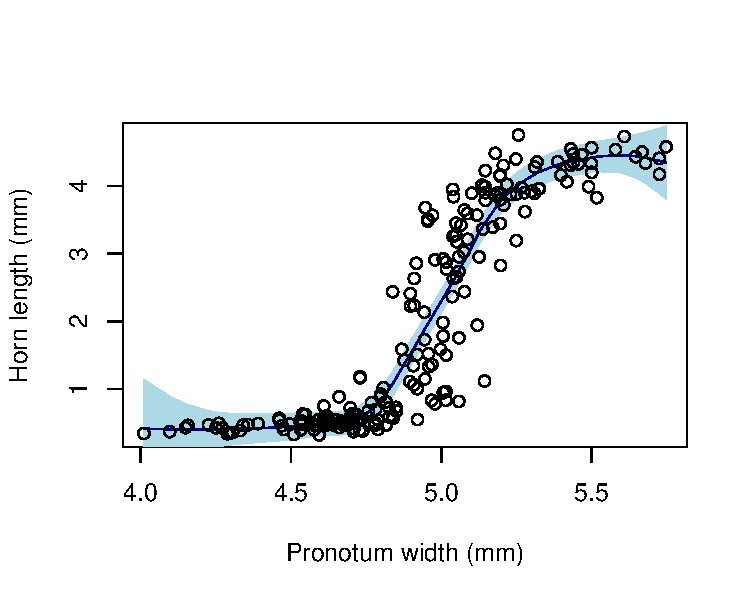
\includegraphics{landUseChangePaper_files/figure-latex/chunk_name-1.pdf}

\begin{longtable}[]{@{}rrr@{}}
\caption{The super result table}\tabularnewline
\toprule
Header 1 & Header 2 & Header 3\tabularnewline
\midrule
\endfirsthead
\toprule
Header 1 & Header 2 & Header 3\tabularnewline
\midrule
\endhead
0.834 & -0.081 & -0.193\tabularnewline
0.338 & 0.085 & 1.012\tabularnewline
-0.890 & 0.371 & -1.912\tabularnewline
1.254 & 0.271 & 0.606\tabularnewline
\bottomrule
\end{longtable}

\subsubsection*{References}\label{references}
\addcontentsline{toc}{subsubsection}{References}

\hypertarget{refs}{}
\hypertarget{ref-aquilueux5fspatialux5f2017}{}
Aquilué, N., De Cáceres, M., Fortin, M.-J., Fall, A. \& Brotons, L.
(2017) A spatial allocation procedure to model land-use/Land-cover
changes: Accounting for occurrence and spread processes.
\emph{Ecological Modelling}, \textbf{344}, 73--86.

\hypertarget{ref-phillipsux5fopeningux5f2017}{}
Phillips, S.J., Anderson, R.P., DudÍk, M., Schapire, R.E. \& Blair, M.E.
(2017) Opening the black box: An open-source release of Maxent.
\emph{Ecography}, n/a--n/a.

\hypertarget{ref-schmuckiux5fregionallyux5f2016}{}
Schmucki, R., Pe'er, G., Roy, D.B., Stefanescu, C., Van Swaay, C.A.,
Oliver, T.H., Kuussaari, M., Van Strien, A.J., Ries, L., Settele, J.,
Musche, M., Carnicer, J., Schweiger, O., Brereton, T.M., Harpke, A.,
Heliölä, J., Kühn, E. \& Julliard, R. (2016) A regionally informed
abundance index for supporting integrative analyses across butterfly
monitoring schemes. \emph{Journal of Applied Ecology}, \textbf{53},
501--510.


\end{document}
